\documentclass[11pt, a4paper]{article}

%%%%%%%%%%%%%%%%%
% Configuration %
%%%%%%%%%%%%%%%%%
\usepackage{allrunes}
\usepackage{amsmath}
% If magyar is wanted
% \usepackage[magyar]{babel}
\usepackage[T1]{fontenc}
\usepackage[utf8]{inputenc}
\usepackage{fixltx2e}
\usepackage{multirow}
\usepackage{url}
\usepackage{amsfonts}
\usepackage{amsthm}
\usepackage{mathtools}
\usepackage{amssymb}
\usepackage{xcolor}

% feynman diagrams
\usepackage{tikz-feynman}

% using circled symbols
\usepackage{tikz}
\newcommand*\circled[1]{\tikz[baseline=(char.base)]{
            \node[shape=circle,draw,inner sep=2pt] (char) {#1}}}


% Here you can configure the layout
\usepackage{geometry}
\geometry{top=1cm, bottom=1cm, left=1.25cm,right=1.25cm, includehead, includefoot}
\setlength{\columnsep}{7mm} % Column separation width

\usepackage{graphicx}

%\usepackage{gensymb}
\usepackage{float}

% For bra-ket notation
\usepackage{braket}

% To have a good appendix
\usepackage[toc,page]{appendix}

\usepackage{abstract}
\renewcommand{\abstractnamefont}{\normalfont\bfseries}
\renewcommand{\abstracttextfont}{\normalfont\small\itshape}
\usepackage{lipsum}

%%%%%%%%%%%%%%%%%%%
% Custom commands %
%%%%%%%%%%%%%%%%%%%
\newcommand{\bb}[1]{\mathbf{#1}}
\newcommand{\dd}{\mathrm{d}}
\newcommand{\Tr}[1]{\mathrm{Tr}\left[#1\right]}
\newcommand{\Sp}[1]{\mathrm{Sp}\left[{#1}\right]}

% \newtheorem*{tetel*}{Tétel}
% \newtheorem*{defn*}{Definíció}
% \newtheorem*{pld*}{Példa}
% \newtheorem*{megj*}{Megjegyzés}
% \newtheorem*{allit*}{Állítás}

% \newtheorem{tetel}{Tétel}
% \newtheorem{defn}{Definíció}
% \newtheorem{pld}{Példa}
% \newtheorem{megj}{Megjegyzés}
% \newtheorem{allit}{Állítás}

% Hyperref should be generally the last package to load
% Any configuration that should be done before the end of the preamble:

\usepackage{hyperref}
\hypersetup{colorlinks=true, urlcolor=blue, linkcolor=blue, citecolor=blue}

\title{Flowering date prediction for bulbous perennials}

\author{Dániel Nagy$^1$,\\Imre M. Jánosi$^2$}
\vspace{2.0cm}
\date{%
    $^1$Institute for Physics, Eötvös Loránd University, H-1117, Pázmány Péter sétány 1/A. Budapest, Hungary\\%
    $^2$Department of Physics of Complex Systems, Eötvös Loránd University, H-1117, Pázmány Péter sétány 1/A. Budapest, Hungary\\[2ex]%
    \today
}

\begin{document}
\maketitle
\vspace{2.5cm}
\begin{figure}[H]
    \centering
    
\includegraphics[scale=0.3]{images/elte.eps}
\end{figure}
\vspace{0.5cm}

\newpage
\begin{abstract}
    The goal of this project is to efficiently predict the first flowering date of bulbous perennials and to identify,
    which meteorological parameters affect the flowering dates. The LSCD model is briefly presented, and the hyperparameters
    of the simpler LSC model are fitted using Gaussian process optimization. A neural network approach for the
    prediction of flowering dates is presented.
\end{abstract}

\section*{Introduction}
\par Many observations prove that plants have a complex sense of climate, and that many of them developed the ability
to prevent premature flowering.
In order to uncover the relationship between meteorological data and flowering time, a long-term data acquisition was needed.
The data available to my project is a \texttt{csv} file that is containing the first flowering dates of 329 bulbous perennial plants 
in the period 1968-2001. Further meteorological data is downloaded from the internet. The most significant meteorological parameter 
is the temperature of the soil at a depth of around 10cm. The temperature data is shown on \ref{fig:tempdata}.
\begin{figure}[H]
    \centering
    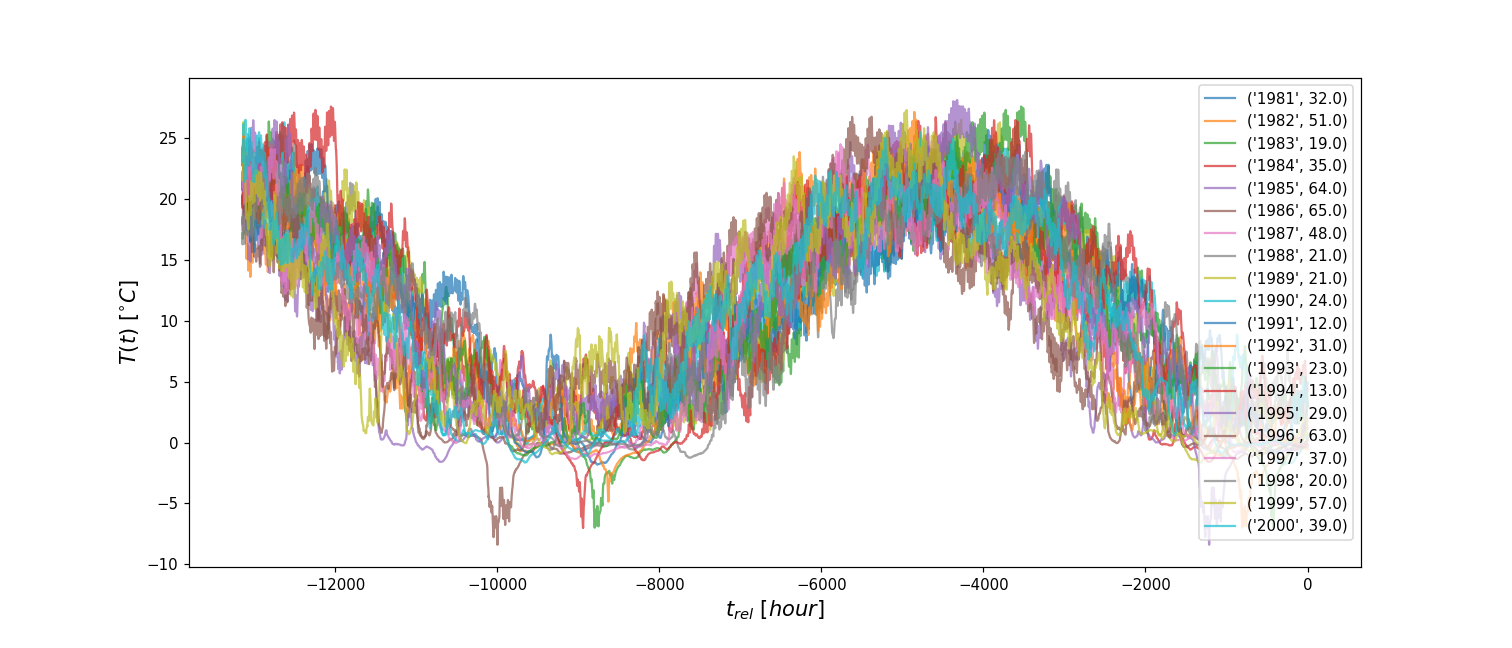
\includegraphics[width=0.75\textwidth]{images/temp_plot.png}
    \caption{The soil temperature at 10cm depth across 22 years, plotted yearly at a 1-hour resolution.
    The x axis shows the hours before flowering date starting from 0.}
    \label{fig:tempdata}
\end{figure}

\section*{The LSCD model}

\begin{equation}
    \frac{\mathrm d\nu}{\mathrm d t} = p_{\nu}(L, S, C, D) - s_{\nu}\nu
\end{equation}
\begin{equation}
    \frac{\mathrm dV}{\mathrm dt} = s_{\nu}\nu - d_VV
\end{equation}
$p_{\nu}(L, S, C, D)=L\cdot S\cdot C\cdot D$ is the productive transcription,
$s_{\nu}$ is the splicing rate, and $d_V$ is the degradation rate of the spliced VIN3.

\begin{equation}
    \frac{\mathrm dL}{\mathrm dt} =
    \begin{cases}
    1-d_LL & T < T_L \\
    -d_LL & T \geq T_L
    \end{cases}
\end{equation}

\begin{equation}
    C(T) =
    \begin{cases}
    p_{c1} & T \leq T_{c1} \\
    p_{c1}-p_{c2}\frac{T-T_{c1}}{T_{c2}-T_{c1}} & T_{c1} < T < T_{c2} \\
    p_{c2} & T \geq T_{c2}
    \end{cases}
\end{equation}

\begin{equation}
    S(T_m) = 
    \begin{cases}
    1, & T < T_S \\
    S_1, & T \geq T_S
    \end{cases}
\end{equation}

\begin{equation}
    D(t) =  \left[p_D + \sin\left(2\pi\left(t - \frac{t_m-1}{24}\right)\right)\right]^2
\end{equation}
$T_m$ is the maximum temperature since the last resetting, which was chosen to occur each day at 4pm.
$t_m$ is the time at dawn.

\begin{figure}[H]
    \centering
    \begin{minipage}{0.4\textwidth}
        \centering
        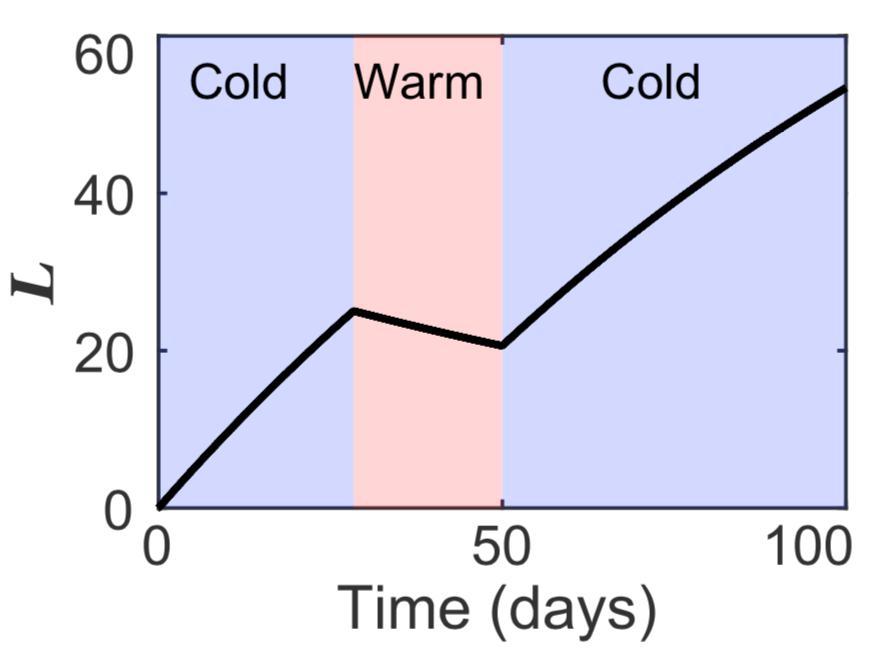
\includegraphics[width=1.0\textwidth]{./images/param_L.png}
        \caption{$L$ intermediator for a }
    \end{minipage}
    \hfill
    \begin{minipage}{0.4\textwidth}
        \centering
        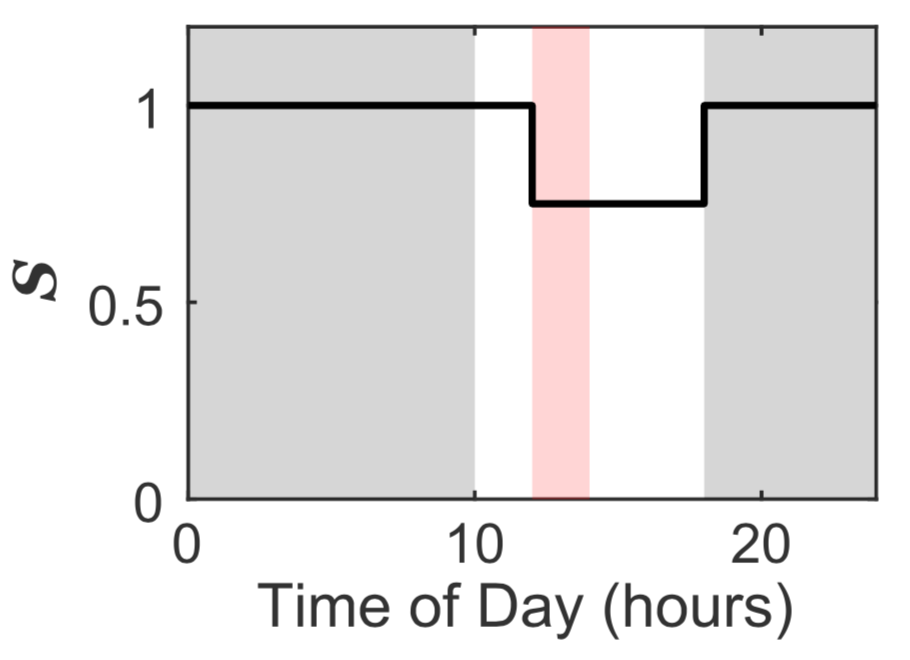
\includegraphics[width=1.0\textwidth]{./images/param_S.png}
    \end{minipage}
\end{figure}
\begin{figure}[H]
    \centering
    \begin{minipage}{0.4\textwidth}
        \centering
        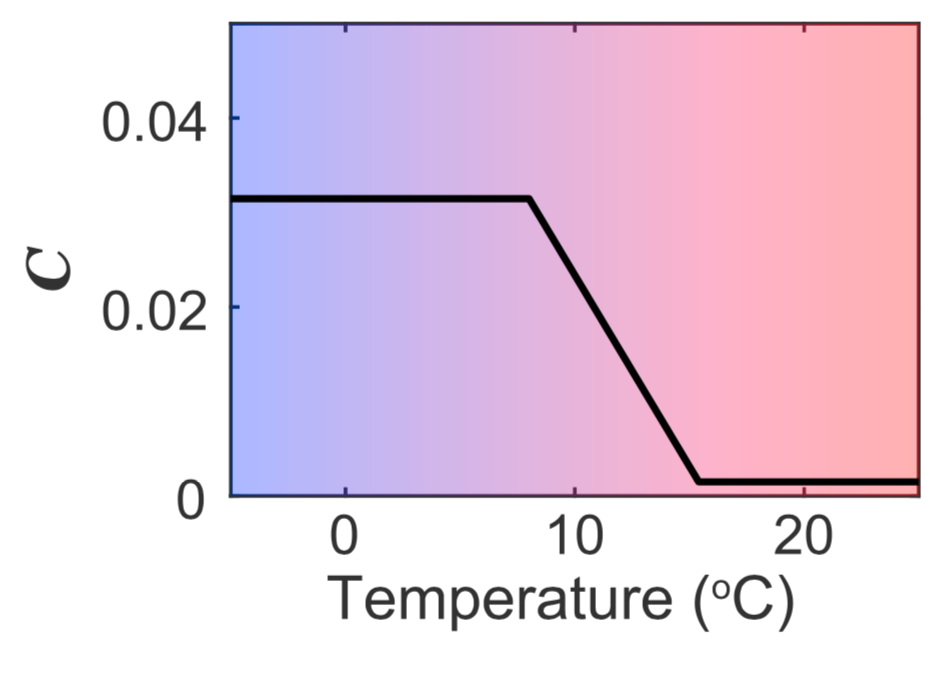
\includegraphics[width=1.0\textwidth]{./images/param_C.png}
    \end{minipage}
    \hfill
    \begin{minipage}{0.4\textwidth}
        \centering
        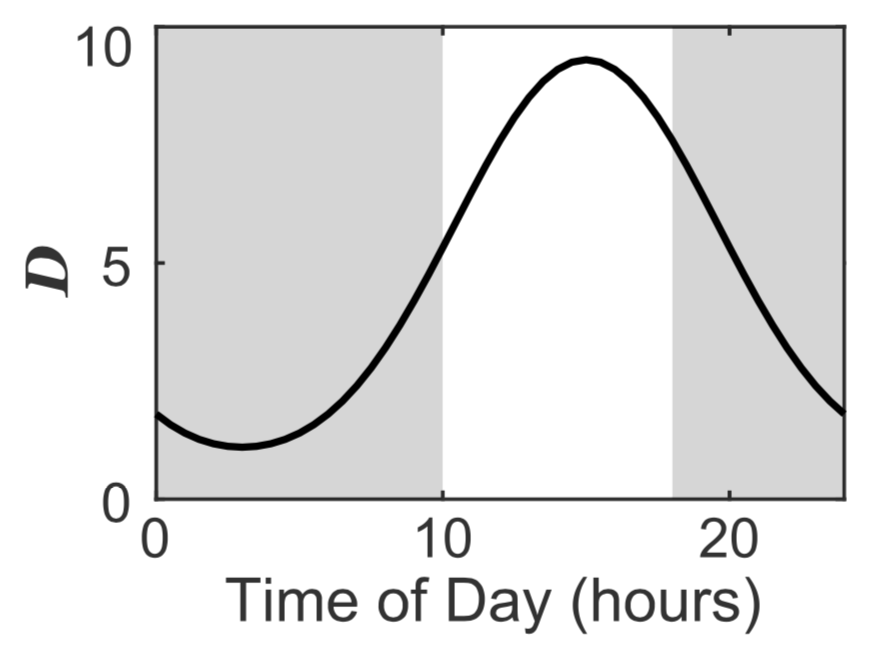
\includegraphics[width=1.0\textwidth]{./images/param_D.png}
    \end{minipage}
\end{figure}

\subsection*{Results with the LSCD model}
\begin{figure}[H]
    \centering
    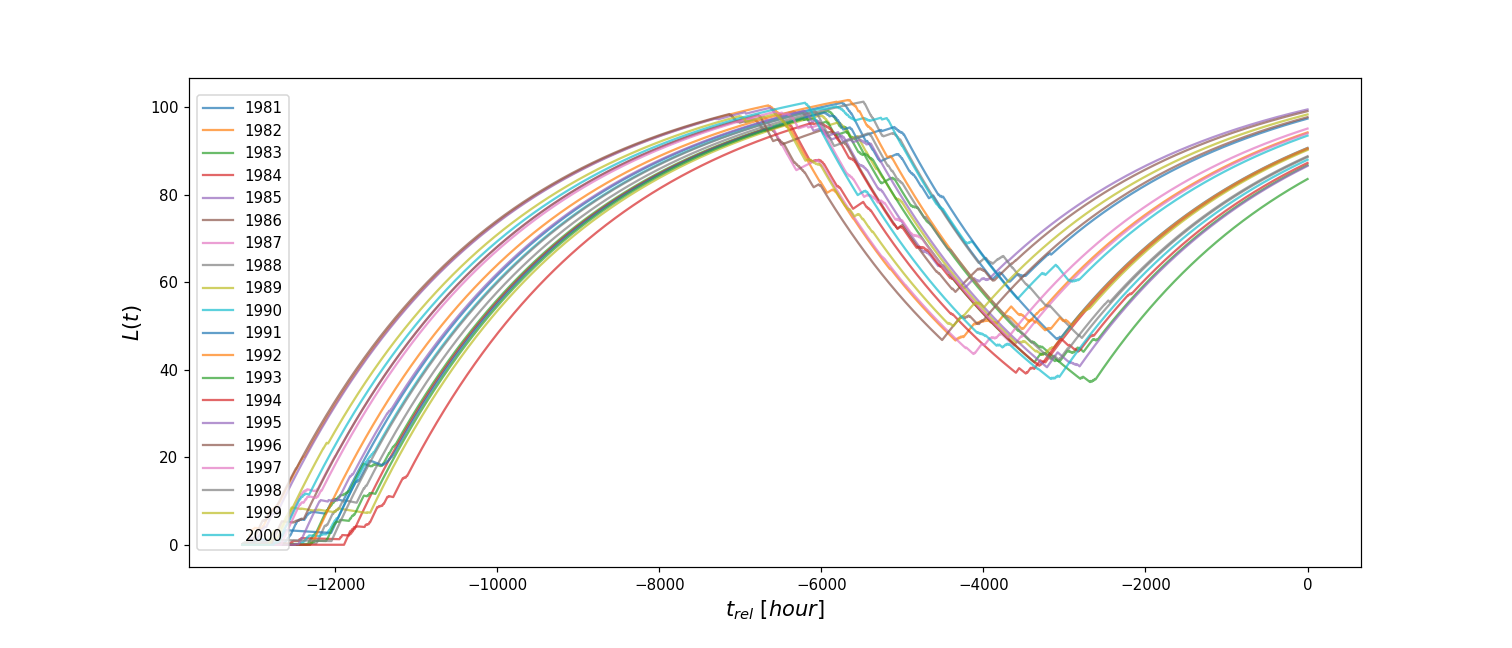
\includegraphics[width=0.75\textwidth]{images/L_plot.png}
\end{figure}
\begin{figure}[H]
    \centering
    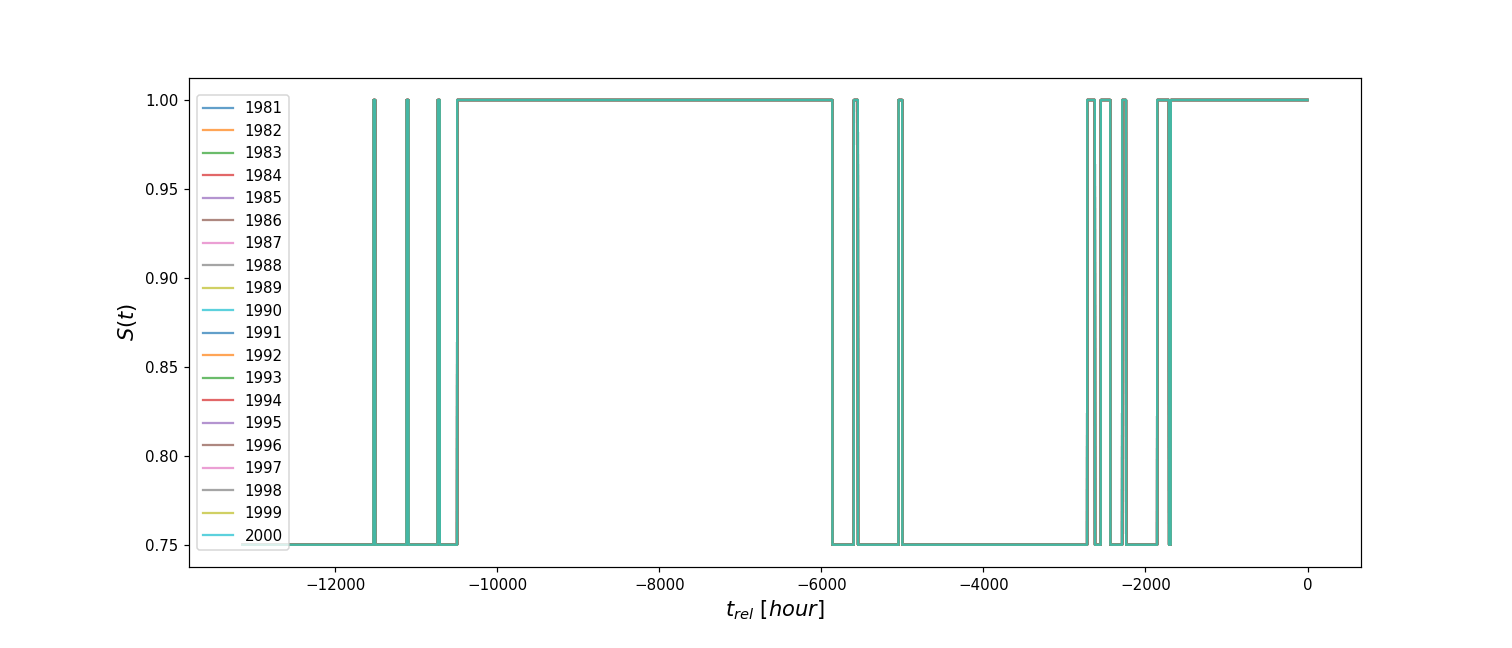
\includegraphics[width=0.75\textwidth]{images/S_plot.png}
\end{figure}
\begin{figure}[H]
    \centering
    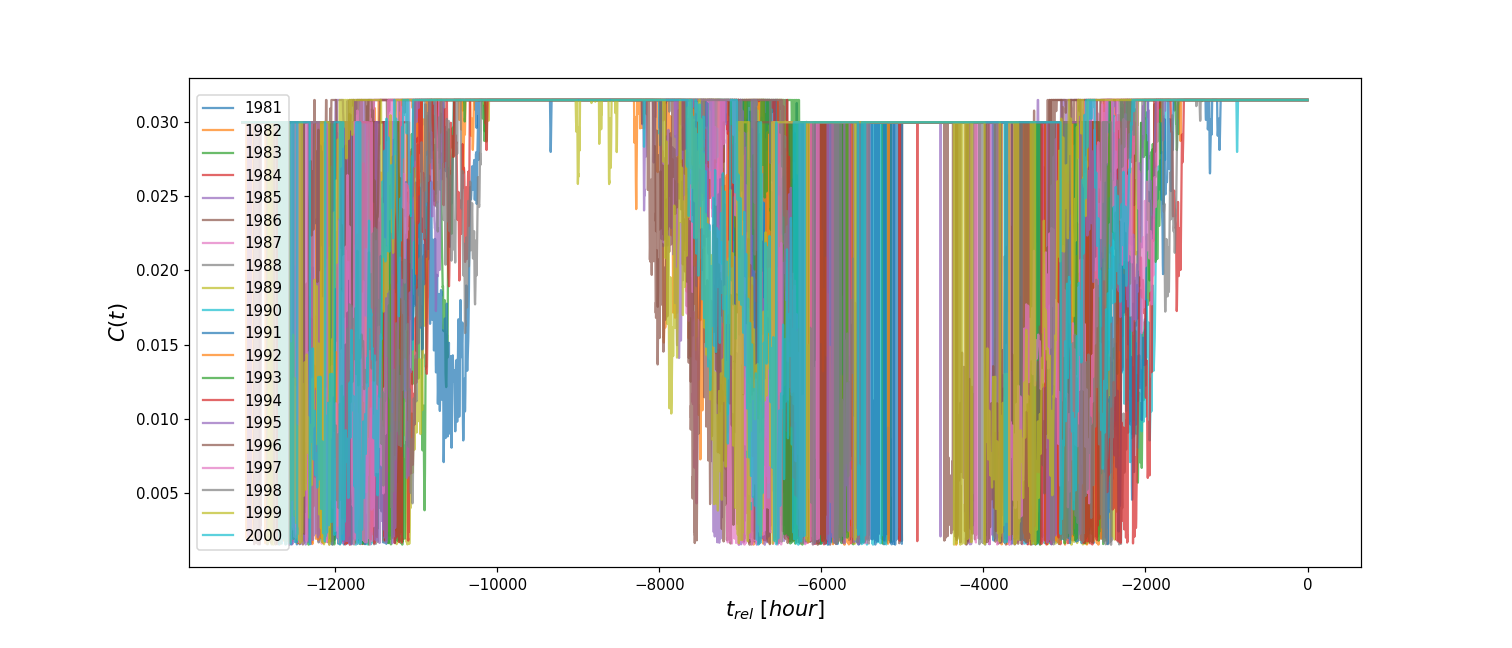
\includegraphics[width=0.75\textwidth]{images/C_plot.png}
\end{figure}
\begin{figure}[H]
    \centering
    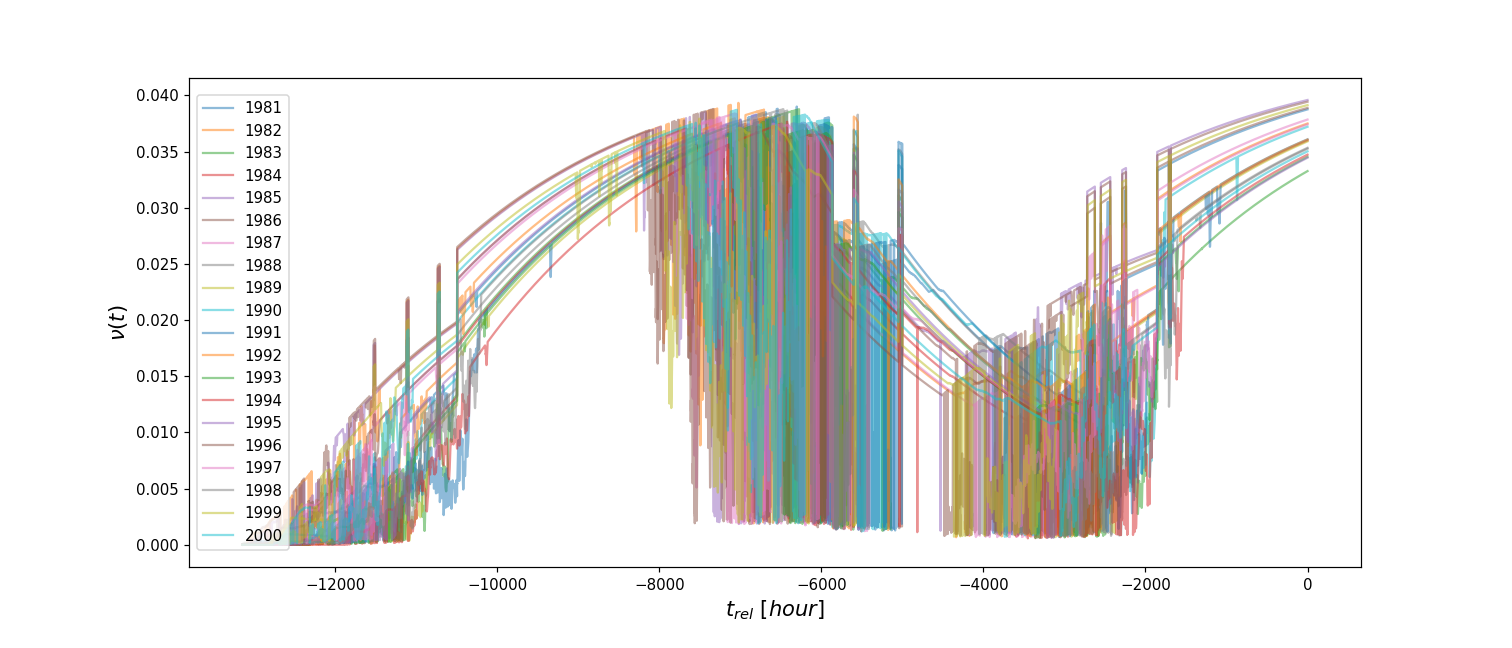
\includegraphics[width=0.75\textwidth]{images/nu_plot.png}
\end{figure}

\begin{figure}[H]
    \centering
    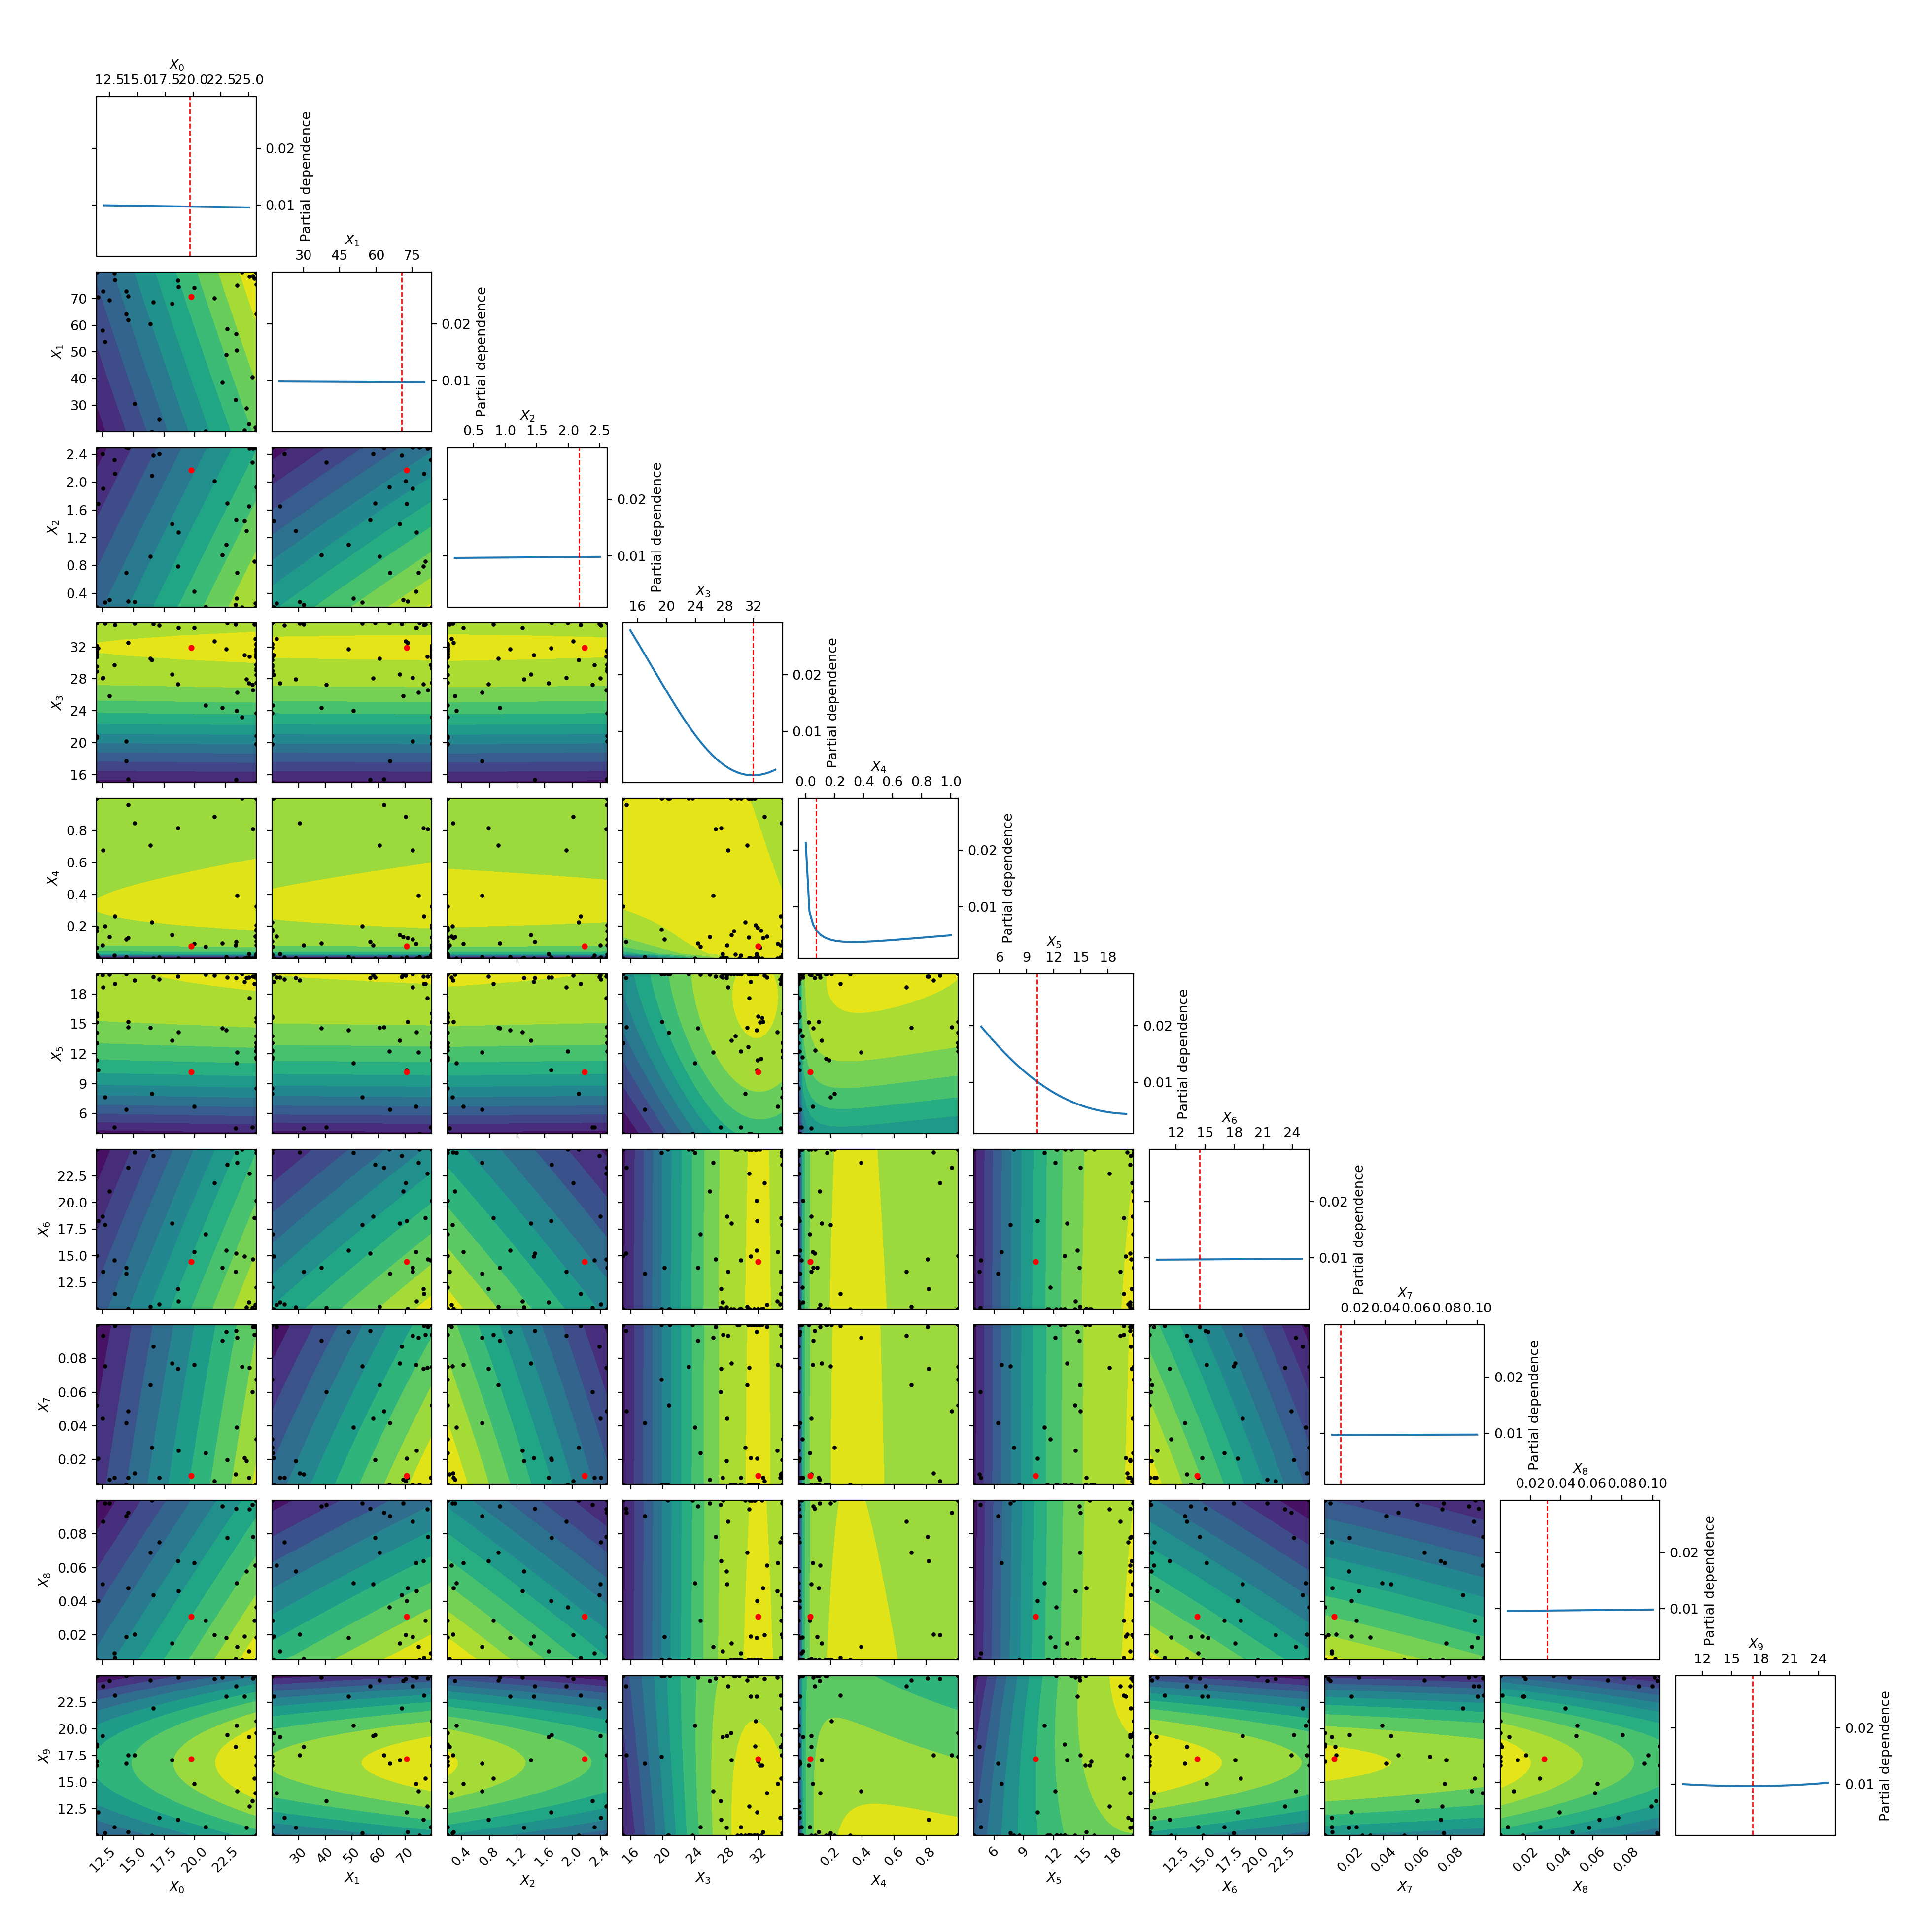
\includegraphics[width=0.99\textwidth]{images/LSC_skopt_objective.png}
\end{figure}

\begin{figure}[H]
    \centering
    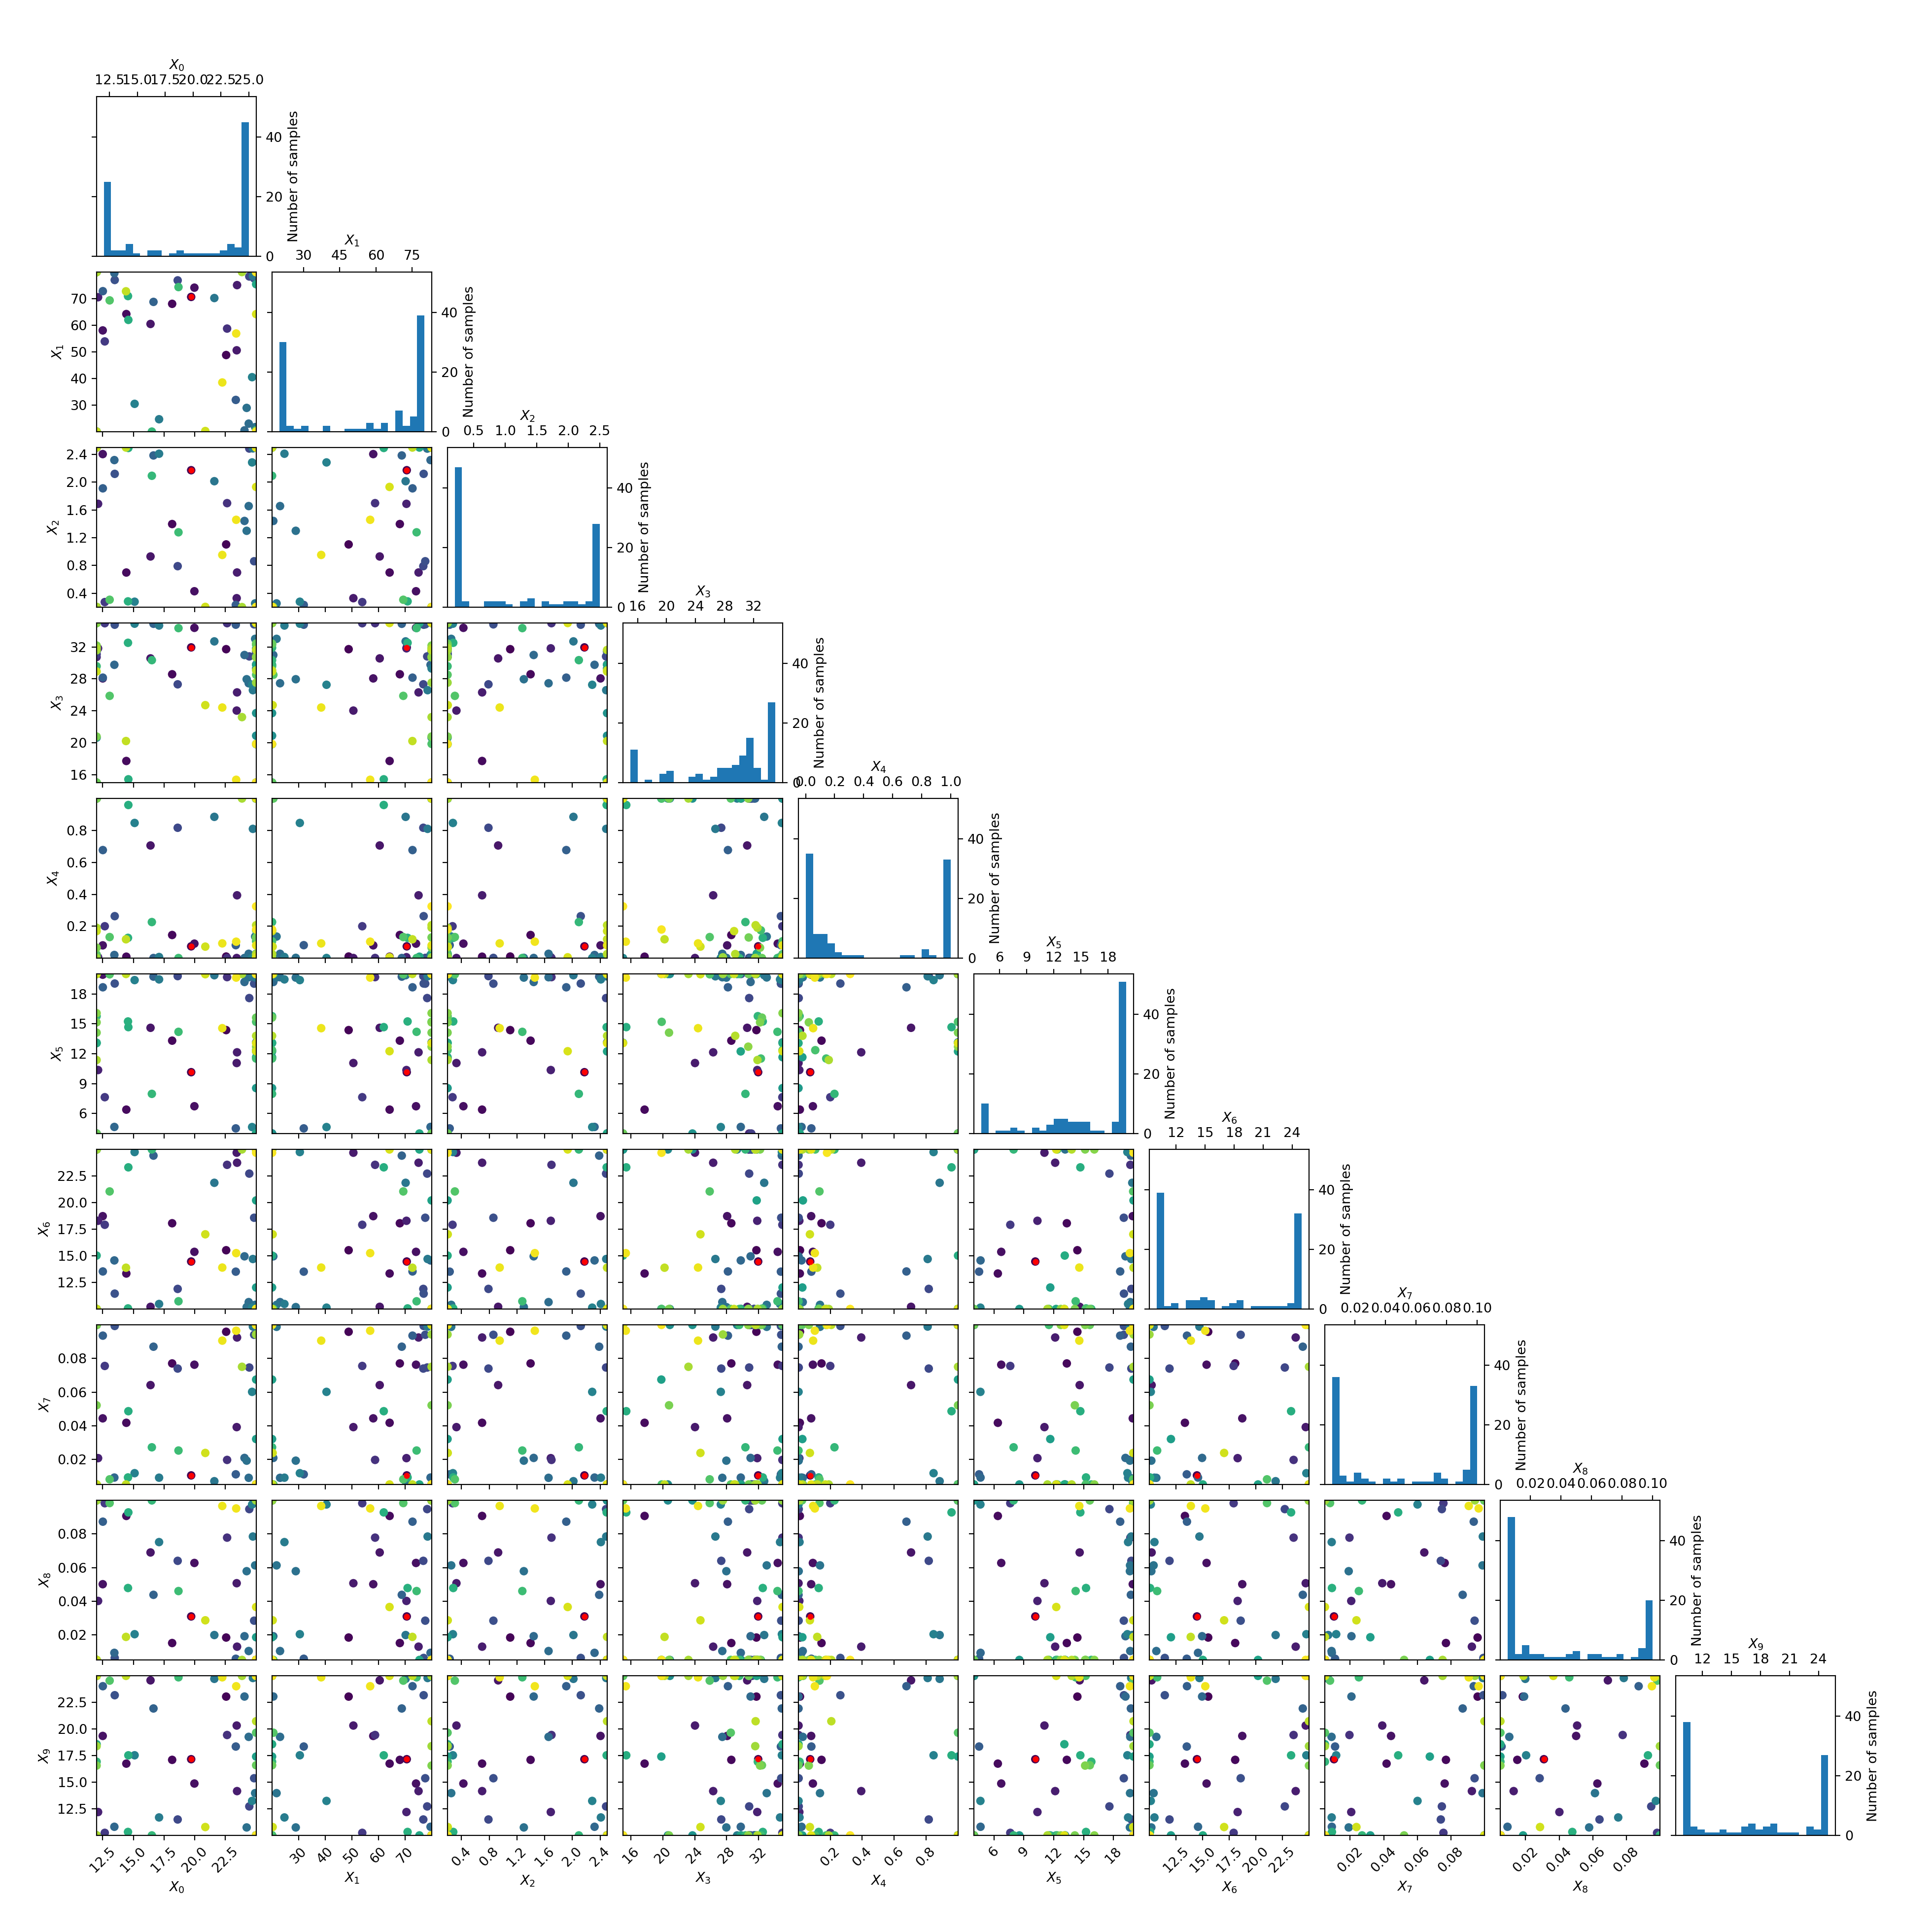
\includegraphics[width=0.99\textwidth]{images/LSC_skopt_evals.png}
\end{figure}


\newpage
\section*{Neural network approach}
\begin{figure}[H]
    \centering
    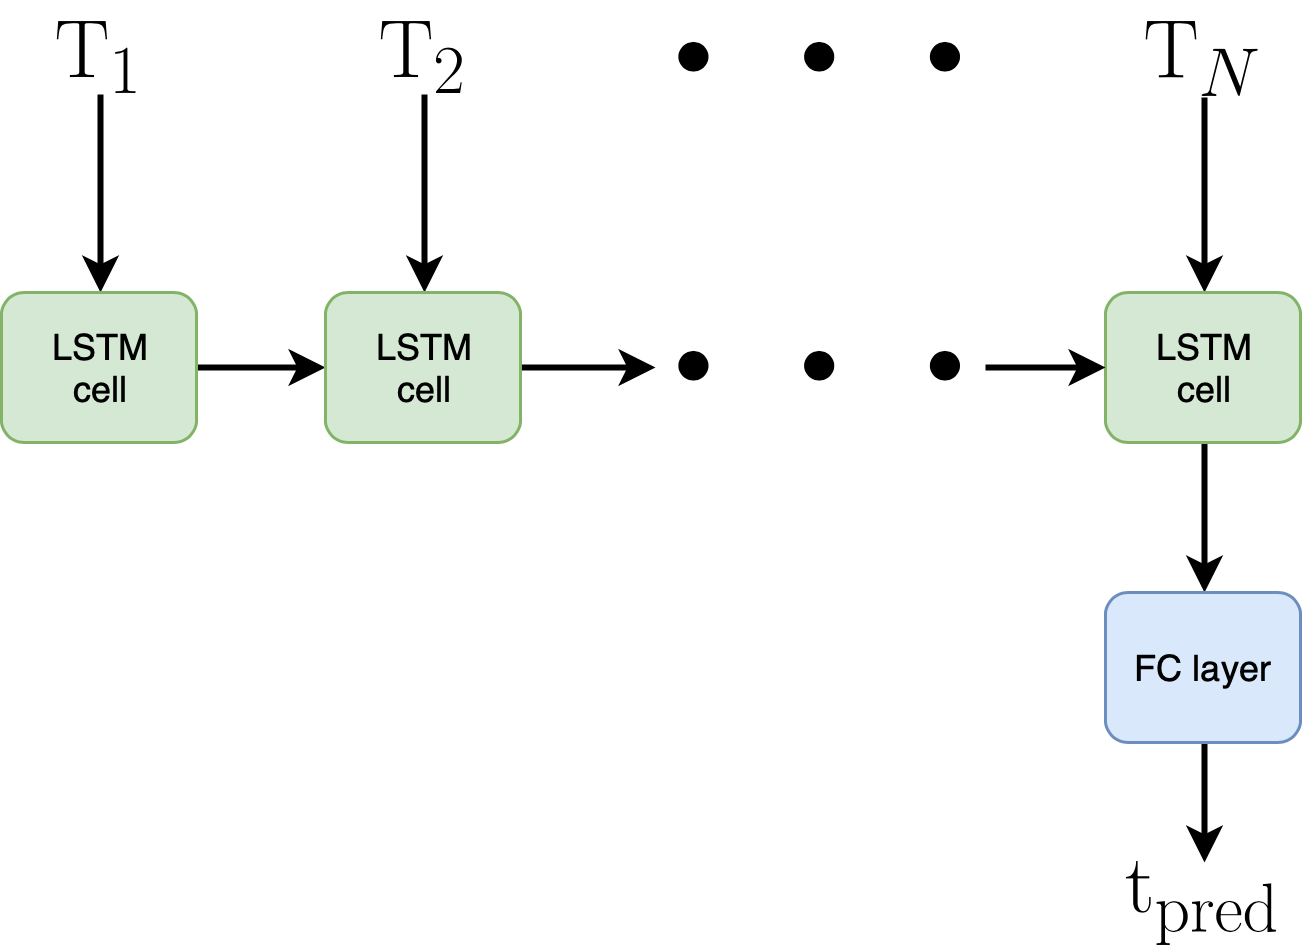
\includegraphics[width=0.65\textwidth]{images/LSTM_arch.png}
    \caption{LSTM architecture for predicting flowering time from temperature measurement series.}
\end{figure}

\subsection*{Results of the neural network approach}
\begin{figure}[H]
    \centering
    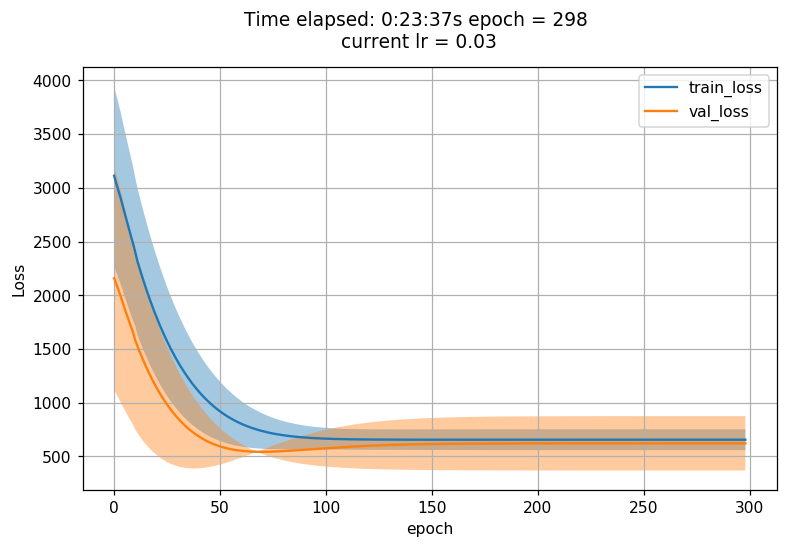
\includegraphics[width=0.75\textwidth]{images/loss-6.png}
\end{figure}


\end{document}